% !TeX spellcheck = cs_CZ
%{\tikzset{external/prefix={tikz/FYZI/}}
% \tikzset{external/figure name/.add={ch50_}{}}
%---------------------------------------------------------------------------------------------------
% file fey1ch50.tex
%---------------------------------------------------------------------------------------------------
%=========================== Kapitola: Harmonické kmity ============================================
\setchaptertoc
\chapter{Harmonické kmity}\label{fyz:IchapL}

\section{Hudební tóny}\label{fyz:IchapLsecI}
  Říká se, že to byl Pythagoras, kdo objevil tento jev. Pro ucho je libozvučné současné znění 
  dvou stejných a stejně napjatých strun s různými délkami, jsou-li délky těchto strun v poměru 
  malých celých čísel. Je-li poměr délek jedna ku dvěma, odpovídá to v hudbě oktávě. Je-li poměr 
  dva ku třem, odpovídá to intervalu mezi C a G, který se nazývá kvintou. Takové intervaly jsou 
  obecně považovány za „libozvučné“ akordy. 
  
  Pythagoras byl tak unesen tímto objevem, že na něm založil celou školu - nazývala se 
  \emph{pythagorejská} - která mysticky věřila ve velkou moc čísel. Panovalo přesvědčení, že něco 
  podobného se zjistí i pro planety - resp. „sféry“. Proto  se říká „hudba sfér“. Základní 
  myšlenka této teorie spočívala v existenci číselných vztahů mezi orbitami planet nebo mezi 
  jinými objekty v přírodě. Lidé to obvykle považují za projev pověrčivosti Řeků. Položme si však 
  otázku, zda je to tak příliš odlišné od našeho vědeckého zájmu o kvantitativní vztahy. 
  Pythagorův objev byl kromě geometrie prvním příkladem numerického vztahu v přírodě. Muselo to 
  být úžasně překvapující najednou objevit v přírodě fakt vyjádřený jednoduchým číselným vztahem. 
  Jednoduchá měření délky poskytla předpověď o něčem, co zjevně nesouviselo s geometrií,   
  předpověď o tvorbě příjemných zvuků. Tento objev vedl k myšlence, že snad aritmetika a   
  numerická analýza budou vhodnými nástroji pro pochopení přírody. Výsledky moderní vědy 
  potvrzují toto stanovisko.
   
  Pythagorovi se podařilo učinit svůj objev jen díky experimentálnímu pozorování. Přesto na něho, 
  jak se zdá, tento důležitý aspekt nezapůsobil. V opačném případě by totiž rozvoj fyziky začal 
  mnohem dříve. (Snadno se mluví o tom, co někdo kdysi udělal, jak to měl udělat!) 
    
  Všimněme si třetího aspektu tohoto velmi zajímavého objevu: máme co činit se dvěma tóny, které 
  pro ucho příjemně znějí. Můžeme si položit otázku, zda jsme na tom lépe než Pythagoras v 
  poznání, proč jsou našemu uchu příjemné určité tóny. Obecná teorie estetiky od dob Pythagora 
  téměř vůbec nepokročila. V tomto jediném objevu Řeků jsou vlastně tři aspekty: experiment, 
  matematické vztahy a estetika. Fyzici byli úspěšní jen v prvních dvou oblastech. Tato kapitola 
  se bude zabývat současným chápáním Pythagorova objevu. 
    
  Mezi zvuky, které slyšíme, je určitý druh, který nazýváme \textbf{šumem}. Šumu odpovídají 
  jakési nepravidelné kmity ušního bubínku vyvolané nepravidelným kmitáním nějakého blízkého 
  objektu. Kdybychom nakreslili graf závislosti tlaku vzduchu na bubínek (a tedy i posunutí 
  bubínku) na čase, zjistili bychom, že je podobný grafu na obr. \ref{fyz:fig381a}. Takový šum 
  odpovídá zhruba dupotu nohou. Hudební tón má jiný charakter. Hudbu můžeme charakterizovat 
  přítomností více méně setrvávajících tónů - nebo hudebních „not“. (Hudební nástroje však dokážou 
  vytvářet i šum!). Tón může trvat relativně krátkou dobu, jako když stlačíme klávesu klavíru nebo 
  může trvat velmi dlouho, jako v případě flétnisty, který píská dlouhý tón. 
    
  V čem spočívá zvláštnost hudebního tónu z hlediska tlaku vzduchu? Hudební tón se liší od šumu v 
  tom, že jeho graf je periodický. Existuje určitý nepravidelný průběh změny tlaku vzduchu v 
  určitém časovém intervalu, ale tento průběh se pak periodicky opakuje. Příklad závislosti tlaku 
  na čase odpovídající hudebnímu tónu je vidět na obr. \ref{fyz:fig381b}.

  \begin{figure}[ht!] %\ref{fyz:fig381}
    \centering
    \subcaptionbox{\label{fyz:fig381a}}{\luafigure[0.8]{fyz_fig381a.pdf}} \newline
    \subcaptionbox{\label{fyz:fig381b}}{\luafigure[0.8]{fyz_fig381b.pdf}}
    \caption{Tlak jako funkce času a) v případě šumu b) v případě hudebního tónu
             (\cite[s.~673]{Feynman01}).}
    \label{fyz:fig381}
  \end{figure}
  
  Hudebníci obvykle charakterizují hudební tón hlasitostí (silou), výškou a kvalitou. Hlasitost 
  odpovídá velikosti tlakových změn. Výška odpovídá časové periodě opakování základní tlakové 
  funkce. (Nízké tóny mají delší periody než vysoké tóny) Kvalita tónu je charakterizována rozdíly, 
  které slyšíme při znění dvou tónů stejné hlasitosti a výšky. Hoboj, housle nebo soprán rozeznáme 
  i tehdy, když vytvářejí tón stejné výšky. Kvalita souvisí se strukturou periodicky se opakujícího 
  obrazce.
  
  Na chvíli předpokládejme, že zvuk vzniká kmitáním struny. Rozezvučíme-li strunu tak, že ji 
  uprostřed vychýlíme a pustíme, bude její další pohyb určován vlnami, které jsme vybudili. Víme, 
  že takové vlny se budou šířit oběma směry a na koncích se odrazí. Pak budou dlouhou dobu putovat 
  z jednoho konce na druhý. Vlna se bude bez ohledu na to, jak je složitá, periodicky opakovat. 
  Perioda opakování je právě doba \(T\) potřebná k tomu, aby vlna proběhla dvě délky celé struny. 
  Je to doba, kterou potřebuje jakákoliv vybuzená vlna k odrazu od každého konce, návratu do 
  původní polohy a pokračování v původním směru. Doba je stejná pro vlny postupující v jednom nebo 
  druhém směru. Každý bod struny se vrátí do své počáteční polohy po jedné periodě a pak znovu po 
  další periodě atd. Vybuzená zvuková vlna se musí opakovat stejně. Tak můžeme vysvětlit vznik 
  hudebního tónu brnknutím o strunu.
  
\section{Fourierovy řady}\label{fyz:IchapLsecII}
  V předcházející kapitole jsme se seznámili s jiným pohledem na kmitající soustavu. Poznali jsme, 
  že struna má různé mody a každou určitou vibraci podmíněnou počátečními podmínkami můžeme 
  považovat za vhodnou kombinaci několika modů, které kmitají současně. V případě struny jsme 
  zjistili, že normální mody mají frekvence \(\omega_0\), \(2\omega_0\) a \(3\omega_0\), 
  \(\ldots\). Nejobecnější pohyb rozkmitané struny je proto složen ze sinusoidálních kmitů se 
  základní frekvencí \(\omega_0\) dále s druhou harmonickou frekvencí \(2\omega_0\) a dále s třetí 
  harmonickou \(3\omega_0\) a atd. Základní mod se opakuje po každé periodě \(T=2\pi/\omega_0\). 
  Druhý harmonický mod se opakuje pokaždé periodě \(T=2\pi/2\omega_0\). Opakuje se však i po 
  \(T_2=2T_1\), tedy po dvou svých periodách. Podobně se třetí harmonický kmit opakuje po časovém 
  intervalu \(T_1\), který představuje jeho tři periody. Tak vidíme, že struna, kterou jsme 
  rozkmitali, opakuje obrazec svého pohybu s periodou \(T_1\). Tím vytváří hudební tón. 
  
  Dosud jsme mluvili o pohybu struny. Ale zvuk, který je pohybem vzduchu, je vyvolán pohybem 
  struny, a proto i jeho kmity se musí skládat ze stejných harmonických kmitů - i když nemůžeme 
  mluvit o vlastních kmitech vzduchu. I relativní velikost harmonických kmitů může být ve vzduchu 
  jiná než ve struně, hlavně tehdy, je-li struna „vázána“ se vzduchem prostřednictvím ozvučnice. 
  Účinnost této vazby se vzduchem je totiž různá pro různé harmonické kmity. 
  
  Vyjadřuje-li funkce \(f(t)\) časovou závislost tlaku vzduchu v případě hudebního tónu (např. 
  takovou jaká je na obr. \ref{fyz:fig381b}), pak můžeme očekávat, že \(f(t)\) lze vyjádřit jako 
  součet určitého počtu jednoduchých harmonických funkcí času - takových jako je \(\cos\omega t\) 	
  - pro každou z různých harmonických frekvencí. Je-li perioda kmitů \(T\), bude základní úhlová 
  frekvence \(\omega = 2\pi/T\) a harmonické frekvence budou \(2\omega\), \(3\omega\) atd.

  Je to však trochu složitější. Nemůžeme totiž očekávat, že počáteční fáze budou pro všechny 
  frekvence stejné. Musíme proto pracovat s funkcemi typu \(\cos(\omega t + \varphi)\). Je však 
  jednodušší používat pro každou frekvenci sinus i kosinus. Vzpomeňme si, že
  \begin{equation}\label{fyz:eq503}
    \cos(\omega t + \varphi) = \cos\varphi\cos\omega t - \sin\varphi\sin\omega t.
  \end{equation}
   a protože \(\varphi\) je konstanta, můžeme \emph{každý} sinusoidální kmit s frekvencí \(\omega\) 
   vyjádřit jako součet takového členu, který obsahuje \(\cos\omega t\) takového, který obsahuje 
   \(\sin\omega t\).
   
   Tak přicházíme k závěru, že každou funkci \(f(t)\), která je periodická s periodou \(T\) můžeme 
   matematicky vyjádřit ve tvaru
   \begin{alignat}{2}
     f(t) &=a_0                &&                    \nonumber  \\
          &+ a_1\cos\omega t  &&+ b_1\sin\omega t   \nonumber  \\
          &+ a_2\cos2\omega t &&+ b_2\sin2\omega t  \nonumber  \\
          &+ a_3\cos3\omega t &&+ b_2\sin3\omega t  \nonumber  \\
          &+ \quad\ldots      &&+\quad\ldots        \label{fyz:eq504}
   \end{alignat}
   kde \(\omega = 2\pi/T\) a \(a_i\) a \(b_i\) jsou číselné konstanty, které nám říkají s jakou 
   váhou je každá složka kmitů přítomna v kmitu \(f(t)\). Přidali jsme i člen a s nulovou 
   frekvencí, a tak náš vztah je zcela obecný, i když v hudebním tónu je tento člen obvykle nulový. 
   Tento člen představuje posun střední hodnoty zvukového tlaku (tj. posun „nulové“ hladiny). S 
   tímto členem můžeme náš vztah použít pro libovolný případ. Rovnice (\ref{fyz:eq504}) je 
   schematicky znázorněna na obr. \ref{fyz:fig382}. (Amplitudy \(a_n\), \(b_n\), harmonických 
   funkcí musí být vhodně vybrány. Na obrázku jsou jen schématicky znázorněny bez dodržení 
   měřítka.) Řada (\ref{fyz:eq504}) se nazývá \textbf{Fourierova řada} pro \(f(t)\).
   
  \begin{figure}[ht!] %\ref{fyz:fig382}
    \centering
    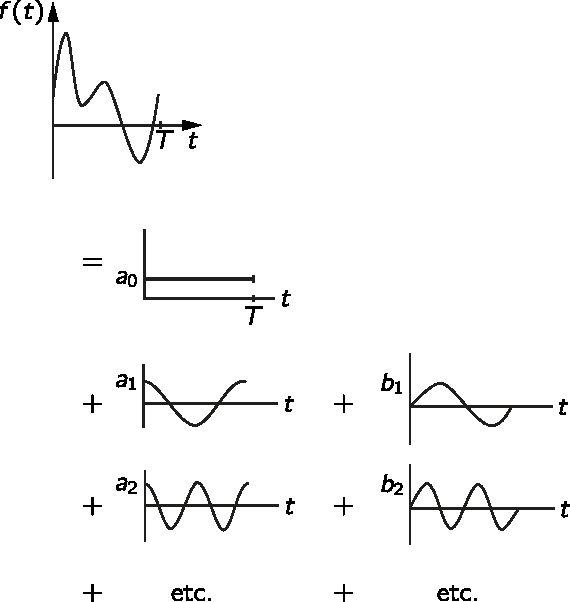
\includegraphics[width=0.8\linewidth]{fyz_fig382.pdf}
    \caption{Libovolná periodická funkce \(f(t)\) je rovna součtu jednoduchých harmonických funkcí
             (\cite[s.~675]{Feynman01})}
    \label{fyz:fig382}
  \end{figure}
  
  Uvedli jsme, že každou periodickou funkci lze takovým způsobem vyjádřit. Toto tvrzení musíme 
  opravit v tom smyslu, že platí pro zvukové vlny nebo pro všechny ty funkce, s nimiž se setkáváme 
  ve fyzice. Matematici však dokážou vymyslet funkce, které nemůžeme složit z jednoduchých 
  harmonických funkcí. Takovým příkladem je funkce, která se „stáčí zpět“, takže má pro některá 
  \(t\) dvě hodnoty. Takové funkce nás však nyní nemusí znepokojovat.
  
\section{Kvalita a libozvučnost}\label{fyz:IchapLsecIII}
  Nyní už můžeme říci, co určuje „kvalitu“ hudebního tónu. Je to relativní množství jednotlivých 
  harmonických, tedy hodnoty koeficientů \(a\) a \(b\), Tón, který obsahuje jen první harmonickou, 
  je „čistý“ tón. Tón, který obsahuje mnoho silných harmonických, je „bohatý“ tón. Housle dávají 
  jiný poměr harmonických tónů než hoboj.
  
  Různé hudební tóny můžeme vytvořit tak, že připojíme k reproduktoru různé oscilátory. (Oscilátor 
  obvykle vytváří téměř čistou jednoduchou harmonickou funkci.) Frekvence oscilátorů můžeme vybrat 
  tak, aby byly \(\omega\), \(2\omega\), \(3\omega\) atd. Pak můžeme nastavením síly každého 
  oscilátoru skládat požadovaná množství jednotlivých harmonických - tak vytvoříme tóny různé 
  kvality. Na tomto principu spočívá činnost elektronického syntezátoru zvuku. Klávesami volíme 
  frekvenci základního oscilátoru a pomocí jezdců ovládáme relativní poměry harmonických. Tak 
  dosáhneme toho, že zvuk varhan zní jako zvuk flétny, hoboje nebo houslí.
  
  Není bez zajímavosti, že k vytvoření takových „umělých“ tónů potřebujeme jen jeden oscilátor pro 
  každou frekvenci - nepotřebujeme oddělené oscilátory pro sinovou a kosinovou složku. Naše ucho 
  totiž není příliš citlivé na relativní fáze harmonických a zaměřuje se hlavně na \emph{celkovou} 
  sinovou a kosinovou část každé frekvence. Naše analýza je tedy přesnější než analýza potřebná 
  k vysvětlení \emph{subjektivního} aspektu hudby. Reakce mikrofonu nebo jiných fyzikálních 
  zařízení však závisí na fázích a naše úplná analýza je pak nezbytná. 
  
  „Kvalita“ řeči je určována zvuky samohlásek, které rozeznáváme v hovoru. Tvar úst určuje 
  frekvenci přirozených modů zvukových vibrací vzduchu v ústní dutině. Některé z těchto modů se 
  vybudí zvukovou vlnou od hlasivek. Takovým způsobem amplitudy některých harmonických zvuků 
  vzrostou proti druhým harmonickým. Změníme-li tvar úst, budou upřednostněny harmonické jiných 
  frekvencí. Tak se vytváří rozdíl mezi zvukem \(e - e - e\) a zvukem \(a - a - a\). 
  
  Všichni dobře víme, že určitá samohláska - řekněme \(e - e - e\) - zůstává stále tou samohláskou, 
  i když ji vyslovujeme (nebo zpíváme) s vyšší nebo nižší frekvencí. Z mechanizmu, který jsme 
  popsali, by se dalo čekat, že při zformování úst pro vyslovení \(e - e - e\) se zdůrazní určité 
  frekvence, které se nesmí změnit při změně výšky našeho hlasu. Pak se však se změnou výšky hlasu 
  musí změnit poměr důležitých harmonických k základní harmonické, musí se tedy změnit kvalita. Je 
  zjevné, že mechanizmus rozeznávání řeči se nezakládá na poměru jednotlivých harmonických. 
  
  Co můžeme nyní říci o Pythagorově objevu? Víme, že dvě podobné struny, jejichž délky jsou v 
  poměru \num{2} ku \num{3}, budou mít základní frekvence v poměru \num{3} ku \num{2}. Proč by ale 
  měly společně příjemně znít? Klíčem k tomuto problému snad budou frekvence vyšších harmonických. 
  Druhá harmonická kratší struny bude mít stejnou frekvenci jako třetí harmonická delší struny. 
  Snadno se ukáže - nebo tomu prostě uvěříme - že brnknutím o strunu vybudíme několik silných 
  nejnižších harmonických. 
  
  Snad bychom mohli zformulovat tato pravidla. Tóny znějí libozvučně, mají-li harmonické se 
  stejnými frekvencemi. Tóny znějí nelibozvučně, mají-li vyšší harmonické málo se lišící frekvence, 
  ale přece jen jsou dost odlišné k tomu, aby mezi nimi vznikly rychlé zázněje. Neumíme popsat, ani 
  definovat, proč zázněje neznějí příjemně, ale souzvuk vyšších harmonických zní příjemně. Na 
  základě našich poznatků neumíme říci, co zní dobře nebo co by mělo například dobře \emph{vonět}. 
  Jinými slovy, naše chápání tohoto jevu není obecnější než pouhé tvrzení, že když znějí tóny 
  unisono, znějí dobře. Nemůžeme z toho však dedukovat nic víc než vlastnosti souladu v hudbě. 
  
  Harmonické vztahy, které jsme popsali, můžeme snadno prověřit jednoduchými experimenty s 
  klavírem. Označme tři po sobě jdoucí noty \(C\) někde ze středu klaviatury symboly \(C\), \(C'\), 
  \(C"\) a tři bezprostředně vyšší noty \(G\) označme symboly \(G\), \(G'\), \(G"\). Základní 
  harmonické budou pak mít následující relativní frekvence:
  \begin{alignat*}{2}
    C  &-2 \quad G  &&-3    \\
    C' &-4 \quad G' &&-6    \\
    C" &-8 \quad G" &&-12.  
  \end{alignat*}
  Tyto harmonické vztahy můžeme demonstrovat takto: \emph{Pomalu} stlačme klávesu \(C'\), takže 
  nezvučí, ale tlumící pedál zdvihneme. Rozezvučíme-li pak \(C\), ozve se základní harmonická i 
  druhá harmonická. Druhá harmonická vybudí kmity struny \(C'\). Uvolníme-li \(C\) (ale \(C'\) 
  ponecháme stlačené), tlumící pedál zastaví kmity struny \(C\) a my slyšíme (měkce) notu \(C'\), 
  jak zaniká. Podobným způsobem může třetí harmonická \(C\) způsobit kmity \(G'\) nebo šestá 
  harmonická \(C\) (která je mnohem slabší) může vybudit kmity základní harmonické \(G"\). 
  
  Poněkud odlišný výsledek dostaneme tehdy, stlačíme-li jemně \(G\) a pak silně \(C'\). Třetí 
  harmonická \(C'\) odpovídá čtvrté harmonické \(G\), takže se vybudí jen čtvrtá harmonická 
  \(G\). Nasloucháme-li pozorně, můžeme slyšet tón \(G"\), který je o dvě oktávy vyšší než \(G\), 
  které jsme stlačili! Není těžké vymyslet mnoho jiných kombinací této hry. Bude na místě 
  poznamenat, že durovou stupnici můžeme definovat právě podmínkou, že každý ze tří durových akordů 
  \((F-A-C)\), \((C-E-G)\) a \((G-B-D)\) představuje posloupnost tónů s frekvenčním poměrem \((4: 
  5:6)\). Tyto poměry - spolu se skutečností, že v oktávě (\(C-C'\), \(B-B'\) atd.) jsou frekvence 
  v poměru \(1:2\) - určují celou stupnici „ideálního“ případu, resp. to, co nazýváme přirozené 
  ladění. Klávesnicové nástroje nebo klavír \emph{nejsou} obvykle laděné tímto způsobem, ale při 
  jejich ladění se dopouštíme malého podvodu, takže frekvence jsou jen přibližně věrné pro všechny 
  možné počáteční tóny. Pro takové ladění, nazývané „temperované“, je oktáva (poměr frekvencí 
  zůstává \(1:2\)) rozdělena na \num{12} stejných intervalů, které mají frekvenční poměr 
  \((2)^{1/12}\). Kvinta už nemá frekvenční poměr \(3/2\), ale \((2)^{7/12} = \num{1.499}\), takže 
  většina lidí tento rozdíl sluchem nepostřehne.
  
  Pomocí shody harmonických frekvencí jsme zformulovali pravidla libozvučnosti v hudbě. Je tato 
  shoda skutečnou \emph{příčinou} libozvučnosti dvou tónů? Jeden vědec tvrdil, že dva čisté tóny - 
  tóny zbavené vyšších harmonických - nevytvoří pocit libozvučnosti nebo nelibozvučnosti, je-li 
  poměr jejich frekvencí přesně nebo přibližně takový jako očekávaný poměr. (Takové experimenty je 
  však těžké uskutečnit, protože je těžké vytvořit čisté tóny z důvodů, o nichž si povíme později.) 
  Nemůžeme s určitostí tvrdit, zda ucho porovnává harmonické nebo používá aritmetiku, když se 
  rozhoduje, zda se nám zvuk líbí.
  
\section{Fourierorvy koeficienty}\label{fyz:IchapLsecIV}
  Vraťme se nyní k myšlence, že každý tón - tj. \emph{periodický} zvuk - můžeme vyjádřit jako 
  vhodnou kombinaci harmonických frekvencí. Chtěli bychom ukázat, v jaké míře jsou jednotlivé 
  harmonické zastoupeny. Jsou-li dány všechny koeficienty \(a\), \(b\), je jednoduché vypočítat 
  \(f(t)\) pomocí rovnice (\ref{fyz:eq504}). Nás však zajímá, jaké jsou pro dané \(f(t)\) 
  koeficienty u jednotlivých harmonických členů. (Je jednoduché upéct koláč podle receptu, ale 
  dokážeme napsat recept, když nám někdo dá ochutnat upečený koláč?)
  
  Fourier přišel na to, že to není příliš složité. Člen \(a_0\) je určitě jednoduchý. Už jsme 
  uvedli, že je to právě střední hodnota \(f(t)\) za jednu periodu (od \(t= 0\) po \(t = T\)). 
  Snadno se o tom můžeme přesvědčit. Střední hodnota sinové nebo kosinové za jednu periodu je 
  nulová. Za dvě nebo tři periody nebo celočíselný násobek periody je také nulová. Proto je střední 
  hodnota všech členů pravé strany rovnice (\ref{fyz:eq504}) nulová kromě členu \(a_0\). (Vzpomeňme 
  si, že musíme zvolit \(\omega = 2\pi/T\))
  
  Střední hodnota součtu je rovna součtu středních hodnot. Proto je střední hodnotou \(f(t)\) právě 
  střední hodnota z \(a_0\). Jenže \(a_0\) je konstanta a její střední hodnota je jí právě rovna. 
  Připomeneme-li si definici střední hodnoty, můžeme psát
  \begin{equation}\label{fyz:eq505}
    a_0 = \frac{1}{T}\int_0^Tf(t)\dd{t}.
  \end{equation}
  Určit ostatní koeficienty není o moc těžší. K jejich určení použijeme trik objevený Fourierem. 
  Násobme obě strany rovnice (\ref{fyz:eq504}) nějakou harmonickou funkcí, řekněme \(\cos7\omega 
  t\). Tak dostaneme
   \begin{alignat}{2}
     f(t)\cdot\cos 7\omega t
         &=a_0\cdot\cos 7\omega t               &&                                      \nonumber \\
         &+ a_1\cos\omega  t\cdot\cos 7\omega t &&+ b_1\sin \omega t\cdot\cos 7\omega t \nonumber \\
         &+ a_2\cos2\omega t\cdot\cos 7\omega t &&+ b_2\sin2\omega t\cdot\cos 7\omega t \nonumber \\
         &+ \quad\ldots                         &&+\quad\ldots                          \nonumber \\
         &+ a_7\cos7\omega t\cdot\cos 7\omega t &&+ b_7\sin7\omega t\cdot\cos 7\omega t \nonumber \\
         &+ \quad\ldots                         &&+\quad\ldots                   \label{fyz:eq506}
   \end{alignat}
  Dále najdeme střední hodnoty obou stran. Střední hodnota \(a_0\cos 7\omega t\) za dobu \(T\) je 
  úměrná střední hodnotě kosinu za \num{7} celých period. Jenže ta je rovna nule. Střední hodnota 
  \emph{téměř všech} ostatních členů je \emph{také} rovna nule. Podívejme se na člen s \(a_1\). 
  Víme, že obecně platí vztah
  \begin{equation}\label{fyz:eq507}
    \cos A\cos B = \frac{1}{2}\cos(A+B) + \frac{1}{2}\cos(A-B).
  \end{equation}
  Člen s \(a_1\) proto lze vyjádřit ve tvaru
  \begin{equation}\label{fyz:eq508}
    \frac{1}{2}a_1(\cos 8\omega t + \cos 6\omega t).
  \end{equation}
  Máme tedy dva kosinové členy, z nichž má jeden osm úplných period \(T\) a druhý šest. 
  \emph{Střední hodnoty obou těchto členů jsou nulové}. Proto je i střední hodnota členu s \(a_1\) 
  nulová. 
  
  Pro člen s \(a_2\) bychom dostali \(a_2\cos9\omega t\) a \(a_2\cos5\omega t\) a střední hodnota 
  každého z těchto členů je nulová. Pro člen s \(a_9\), bychom dostali \(\cos16\omega t\) a 
  \(\cos(-16\omega t)\) je stejný jako \(\cos2\omega t\) a tak střední hodnoty obou těchto členů 
  jsou nulové. Je jasné, že všechny členy s koeficienty \(a\) budou mít nulové střední hodnoty až 
  na jediný člen, který je právě člen s \(a_7\). Pro tento člen dostaneme
  \begin{equation}\label{fyz:eq509}
    \frac{1}{2}a_7(\cos 14\omega t + \cos0).
  \end{equation}
  Kosinus nuly je jedna a taková je i jeho střední hodnota. Přicházíme tak k výsledku, že střední 
  hodnota všech členů rovnice (\ref{fyz:eq506}), které obsahují koeficienty a je rovna \(1/2 a_7\).
  
  Členy s koeficienty \(b\) jsou ještě jednodušší. Násobíme-li je kosinovým výrazem, jako je např.
  \(\cos n\omega t\), stejným způsobem jako předtím, můžeme dokázat, že jejich střední hodnoty budou
  nulové. Je vidět, že Fourierův „trik“ působil jako síto. Při násobení \(\cos 7\omega t\) a 
  zprůměrování, všechny členy vypadly, kromě členu s \(a_7\), a platilo 
  \begin{equation}\label{fyz:eq510}
    \text{Střední hodnota }[f(t)\cdot\cos 7\omega t] = a_7/2,
  \end{equation}
  tedy
  \begin{equation}\label{fyz:eq511}
    a_7 = \frac{2}{T}\int_0^Tf(t)\cdot\cos7\omega t \dd{t}.
  \end{equation}
   Není těžké dokázat, že koeficient \(b_7\), můžeme získat násobením rovnice (\ref{fyz:eq504}) 
   výrazem \(\sin 7\omega t\) a vyjádřením střední hodnoty obou stran rovnice. Tak získáme výsledek
  \begin{equation}\label{fyz:eq512}
    b_7 = \frac{2}{T}\int_0^Tf(t)\cdot\sin7\omega t \dd{t}.
  \end{equation}
  To, co platí pro číslo \num{7}, zřejmě platí pro libovolné celé číslo. Výsledek našeho důkazu 
  můžeme shrnout do následujícího elegantnějšího matematického tvaru. Jsou-li \(m\) a \(n\) celá 
  čísla různá od nuly a je-li \(\omega = 2\pi/T\), pak
  \begin{equation}\label{fyz:eq513}
    \int_{0}^{T}\sin n\omega t\cos m\omega t\dd{t} = 0
  \end{equation}
  \begin{equation}\label{fyz:eq514}
    \left.\begin{aligned}
           \int_{0}^{T}\cos n\omega t\cos m\omega t\dd{t} &= \\
           \int_{0}^{T}\sin n\omega t\sin m\omega t\dd{t} &=
          \end{aligned}
    \right\}
    \begin{cases} 
       0             & \text{pro } n \neq m \\
       \dfrac{T}{2}  & \text{pro } n = m
    \end{cases}
  \end{equation}
  \begin{equation}\label{fyz:eq515}
    f(t) = a_0 + \sum_{n=1}^\infty a_n\cos n\omega t + \sum_{n=1}^\infty b_n\sin n\omega t
  \end{equation}
  \begin{subequations}\label{fyz:eq516}
    \begin{align}
      a_0 &= \dfrac{1}{T}\int_{0}^{T}f(t)\dd{t}  \\
      a_n &= \dfrac{1}{T}\int_{0}^{T}f(t)\cos n\omega t\dd{t}   \\
      b_n &= \dfrac{1}{T}\int_{0}^{T}f(t)\sin n\omega t\dd{t}. 
    \end{align}
  \end{subequations}
  V předcházejících kapitolách bylo výhodné popisovat jednoduchý harmonický pohyb pomocí 
  exponenciální funkce. Místo \(\cos\omega t\) jsme psali \(e^{i\omega t}\), tedy reálnou část 
  exponenciální funkce. V této kapitole jsme pracovali se sinem a kosinem, protože tak se stal náš 
  důkaz trochu přehlednější. Náš konečný výsledek, rovnice (\ref{fyz:eq515}), však lze vyjádřit v 
  kompaktnější formě
  \begin{equation}\label{fyz:eq517}
    f(t) = Re\sum_{n=0}^{\infty}\hat{a}_n e^{in\omega t}
  \end{equation}
  kde \(\hat{a}\) je komplexní číslo \(a_n - ib_n\), (přičemž \(b_0 = 0\)). Kdybychom chtěli takový 
  zápis používat důsledně, museli bychom psát
  kompaktnější formě
  \begin{equation}\label{fyz:eq518}
    \hat{a}_n = \dfrac{1}{T}\int_{n=0}^{T}f(t) e^{-in\omega t}\dd(t)\quad (n\geq1)
  \end{equation}
  Nyní už umíme rozložit periodickou vlnu na její harmonické složky. Takový postup se nazývá rozvoj 
  do \textbf{Fourierovy řady} a jednotlivé členy se nazývají \emph{Fourierovými složkami}. 
  Neukázali jsme však, že určením všech Fourierových složek a jejich sčítáním se dostaneme opravdu 
  zpět k naší funkci \(f(t)\). Matematici dokázali pro širokou třídu funkcí, vlastně pro všechny 
  ty, které zajímají fyziky, že umíme-li vypočítat požadované integrály, dostaneme se nazpět k 
  \(f(t)\). Je zde však jedna malá výjimka. Je-li funkce \(f(x)\) nespojitá, tj. když najednou 
  skočí z jedné hodnoty na druhou, Fourierův součet dá v bodě nespojitosti hodnotu, která leží 
  uprostřed mezi dolní a horní hodnotou skutečné funkce v tomto bodě. Kdybychom tedy měli takovou 
  zvláštní funkci: \(f(t) = 0, 0 \leq t<t_0\) a \(f(t) = 1 pro t_0 \leq t \leq T\), Fourierova řada 
  by dala správnou hodnotu všude kromě bodu \(t_0\), kde by dala hodnotu \num{1/2} místo \num{1}. 
  Je však dost nefyzikální požadovat, aby funkce byla nulová až po \(t_0\) a jednotková 
  \emph{právě} v \(t_0\).  Snad by bylo přece jen dobré pro fyziky formulovat „pravidlo“ tak, že 
  každá nespojitá funkce (která může být jen zjednodušením skutečné fyzikální funkce) musí nabývat 
  v bodě nespojitosti hodnotu, která leží uprostřed hodnot, jež má funkce zleva a zprava. Pak každá 
  taková funkce - s libovolným počtem skoků - bude stejně jako ostatní fyzikálně zajímavé funkce 
  správně určována Fourierovou řadou.
    
  \begin{figure}[ht!] %\ref{fyz:fig383}
    \centering
    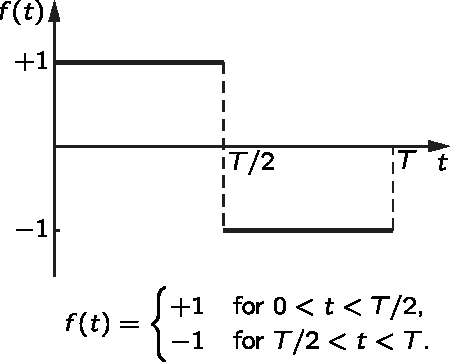
\includegraphics[width=0.6\linewidth]{fyz_fig383.pdf}
    \caption{Skoková funkce
             (\cite[s.~680]{Feynman01})}
    \label{fyz:fig383}
  \end{figure}
  
  Jako cvičení můžeme určit Fourierovu řadu pro případ funkce znázorněné na obr. \ref{fyz:fig383} 
  Vzhledem k tomu, že funkci nemůžeme vyjádřit v explicitním algebraickém tvaru, nebude možné 
  počítat integrály od \num{0} po \(T\) obvyklým způsobem. Integrály jsou však jednoduché, 
  rozdělíme-li je na dvě části: integrál od \num{0} po \(T/2\) (kde je \(f(t) = 1\)) a na integrál 
  od \(T/2\) do \(T\) (kde je \(f(t) = - 1\)). Tak musíme dostat
  
  \begin{equation}\label{fyz:eq519}
    f(t) = \dfrac{4}{\pi}
             \left(
                \sin\omega t + \dfrac{1}{3}\sin3\omega t + \dfrac{1}{5}\sin5\omega t + \ldots
             \right),
  \end{equation}
  kde \(\omega = 2\pi/T\). Pravoúhelníková vlna (se speciálně zvolenou fází) má tedy jen liché 
  harmonické a jejich amplitudy jsou nepřímo úměrné jejich frekvencím. 
  
  Prověřme, zda nás rovnice (\ref{fyz:eq519}) skutečně přivedla nazpět k funkci \(f(t)\) pro 
  některou hodnotu \(t\). Zvolme \(t = T/4\), tedy \(\omega t = \pi/2\). Tehdy máme
  \begin{align}\label{fyz:eq520}
    f(t) &= \dfrac{4}{\pi}
              \left(
                \sin\dfrac{\pi}{2} + \dfrac{1}{3}\sin\dfrac{3\pi}{2} + 
                \dfrac{1}{5}\sin\dfrac{5\pi}{2} + \ldots
              \right),                \nonumber \\
         &= \dfrac{4}{\pi}
              \left(
                1 - \dfrac{1}{3} + \dfrac{1}{5} - \dfrac{1}{7} + \ldots
              \right)
  \end{align}
  Součet takové řady je však znám\footnote{Součet této řady můžeme vypočítat následujícím způsobem. 
  Nejprve si uvědomme, že \(\int_0^x[\dd{x}/(1+x^2)]=\arctg x\). Dále rozložme podintegrální výraz 
  do 
  řady \(1/(1+x^2) = 1 - x^2 + x^4 - x^6 + \ldots\). Integrujeme-li tuto řadu tak, že integrujeme 
  každý člen zvlášť (v intervalu od \num{0} po \(x\)), dostaneme \(\arctg x = 1 - x^3/3 + x^5/5 - 
  x^7/7\). Položíme-li \(x = 1\), dostaneme hledaný vztah, neboť \(\arctg 1 = \pi/4\).} a je roven 
  \(\pi/4\), takže bude \(f(t) = 1\)
  
\section{Věta o energii}\label{fyz:IchapLsecV}
  Energie vlny je úměrná druhé mocnině její amplitudy. V případě vlny složitého tvaru je energie za 
  jednu periodu úměrná \(\int_0^Tf^2(t)\dd{t}\). Tuto energii můžeme dát do souvislosti s 
  Fourierovými koeficienty. Můžeme psát
  \begin{equation*}
    \int\limits_0^Tf^2(t)\dd{t} = \int\limits_0^T
      \left[a_0 + \sum_{n=1}^\infty a_n\cos n\omega t +
                  \sum_{n=1}^\infty b_n\sin n\omega t
      \right]^2\dd{t}.
  \end{equation*}
  Vyjádříme-li druhou mocninu výrazu v závorce, dostaneme všechny možné křížové členy. Jeden z nich 
  je například člen \(a_5\cos5\omega t\cdot b_7\sin7\omega t\). Ukázali jsme však už dříve (rovnice 
  (\ref{fyz:eq513}) a (\ref{fyz:eq514})), že integrály všech takových členů přes jednu periodu 
  dávají nulu. Zůstávají nám jen kvadratické členy typu \(a_5^2\cos^2\omega t\). Integrál z druhé 
  mocniny libovolného kosinu nebo sinu přes jednu periodu je rovem \(T/2\), a proto máme
  \begin{align}
    \int\limits_0^Tf^2(t)\dd{t} 
      &= Ta_0^2 + \frac{T}{2}(a_1^2 + a_2^2 + \ldots + b_1^2 + b_2^2 + \ldots)   \nonumber \\
      &= Ta_0^2 + \frac{T}{2}\sum_{n=1}(a_n^2 + b_n^2)                           \label{fyz:eq521}
  \end{align}
  Tato rovnice se nazývá „věta o energii“ a říká, že celková energie vlny je rovna součtu energií 
  všech Fourierových složek. Kdybychom například tuto větu aplikovali na řadu (\ref{fyz:eq519}) a 
  uvážili, že \([f(t)]^2 = 1\), dostali bychom
  \begin{equation}\label{fyz:eq522}
    T = \frac{T}{2}\left(\dfrac{4}{\pi}\right)^2
        \left(1 + \frac{1}{3^2} + \frac{1}{5^2} + \frac{1}{7^2} + \ldots\right),
  \end{equation}
  a tak bychom se dozvěděli, že součet reciprokých druhých mocnin lichých celých čísel je roven 
  \(\pi^2/8\). Kdybychom zapsali podobným způsobem nejprve Fourierovu řadu pro funkci a pak použili 
  větu o energii, mohli bychom dokázat, že \(1 + 1/2^4 + 1/3^4 + \ldots\) je rovno \(\pi^4/90\); 
  tento výsledek jsme potřebovali v \ref{fyz:IchapXLV}. kapitole.
  
\section{Nelineární odezvy}\label{fyz:IchapLsecVI}
  V harmonické teorii je ještě jeden důležitý prvek, na který je třeba upozornit pro jeho praktický 
  význam, a tím jsou nelineární efekty. Ve všech soustavách, které jsme dosud uvažovali, jsme 
  předpokládali linearitu, tedy odezvy na síly, např. výchylky nebo zrychlení byly vždy úměrné 
  silám. Proudy v obvodech byly úměrné napětím apod. Nyní budeme uvažovat takové případy, kde tato 
  přísná úměrnost není. Na chvíli uvažujme nějaký přístroj, v němž odezva - označíme ji \(x_{od}\) 
  - bude v okamžiku \(t\) určována vstupní veličinou \(x_{vs}\), ve stejném okamžiku. Veličinou 
  \(x_{vs}\) může například být síla a \(x_{od}\) může být výchylka nebo \(x_{vs}\) může být proud 
  a \(x_{od}\) napětí. Je-li přístroj lineární, bude
  \begin{equation}\label{fyz:eq523}
    x_{od}(t) = Kx_{vs}(t), 
  \end{equation}
  kde \(K\) je konstanta nezávislá na \(t\) a \(x_{vs}\). Předpokládejme však, že přístroj není 
  přesně lineární, ale jen přibližně, takže můžeme psát  
  \begin{equation}\label{fyz:eq525}
    x_{od}(t) = K[x_{vs}(t) + \varepsilon x_{vs}^2(t)], 
  \end{equation}
  kde \(\varepsilon\) je malé vzhledem k jedné.Takové lineární a nelineární odezvy jsou znázorněné 
  na grafech obrázku \ref{fyz:fig384}.
  
  \begin{figure}[ht!] %\ref{fyz:fig384}
    \centering
    \begin{tabular}{cc}
     \subcaptionbox{Lineární: \newline\(x_{out} = Kx_{in}\)  \label{fyz:fig384a}}
        {\luafigure[0.45]{fyz_fig384a.pdf}}
     \hspace{1cm}
     \subcaptionbox{Nelineární: \newline\(x_{out}=K(x_{in}+\varepsilon x^2_{in})\) \label{fyz:fig384b}}
        {\luafigure[0.45]{fyz_fig384b.pdf}}
    \end{tabular}
    \caption{Lineární a nelineární odezva
             (\cite[s.~682]{Feynman01}).}
    \label{fyz:fig384}
  \end{figure}
  
  Nelineární odezvy mají některé důležité praktické důsledky a o některých z nich si povíme. 
  Nejprve si všimneme, co se stane, připojíme-li na vstup čistý tón. Ať \(x_{vs} = \cos\omega t\). 
  Nakreslíme-li \(x_{od}\) jako funkci času, dostaneme plnou čáru na obr. \ref{fyz:fig385}. 
  Přerušovaná čára je pro porovnání a představuje odezvu lineární soustavy. Je vidět, že na výstupu 
  už nedostáváme kosinovou funkci. Tato funkce je nahoře ostřejší a dole plošší. Říkáme, že 
  výstupní signál je zkreslený. Taková vlna už není čistým tónem a bude obsahovat vyšší harmonické. 
  Zjistíme, které to budou. Dosadíme-li \(x_{vs} = \cos\omega t\) do rovnice (\ref{fyz:eq525}), 
  dostaneme
  \begin{equation}\label{fyz:eq524}
    x_{od} = K[\cos\omega t + \varepsilon\cos^2\omega t ]. 
  \end{equation}
  Využijeme-li známý vztah \(\cos^2\vartheta = \frac{1}{2}(1 - \cos2\vartheta)\), dostaneme 
  \begin{equation}\label{fyz:eq526}
    x_{od} = K\left(\cos\omega t+\frac{\varepsilon}{2}-\frac{\varepsilon}{2}\cos2\omega t\right). 
  \end{equation}
  Výstupní signál má tedy nejen složku základní frekvence, kterou měli vstupní signál, ale má i 
  určitou část druhé harmonické. Na výstupu se objevuje i konstantní člen \(K(\varepsilon/2)\), 
  který odpovídá posunu střední hodnoty znázorněnému na obr. \ref{fyz:fig385}. Proces vytvoření 
  posunu střední hodnoty se nazývá \emph{usměrnění}
  
  \begin{figure}[ht!] %\ref{fyz:fig385}
    \centering
    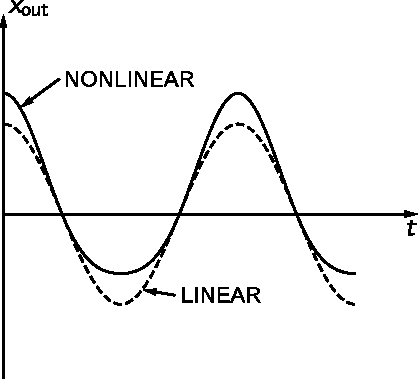
\includegraphics[width=0.6\linewidth]{fyz_fig385.pdf}
    \caption{Odezva nelineárního přístroje na vstupní signál \(\cos\omega t\). Pro porovnání je 
             znázorněna i lineární odezva.
             (\cite[s.~682]{Feynman01})}
    \label{fyz:fig385}
  \end{figure}
  
  Nelineární systém tedy usměrňuje a vytváří vyšší harmonické frekvencí přivedených na vstup, I 
  když nelinearita, kterou jsme uvažovali, vytvářela jenom druhou harmonickou, nelinearity vyššího 
  řádu - například takové, které obsahují členy jako \(x^3\), \(x^4\) - budou vytvářet vyšší 
  harmonické než druhou.
  
  Dalším důsledkem nelineární odezvy je \textbf{modulace}. Obsa\-huje-li náš vstupní signál dva 
  čisté tóny (nebo i více), nedostaneme na výstupu jen jejich harmonické, ale i jiné frekvenční 
  složky. Nechť \(x_{vs} = A\cos\omega_1 t + B\cos\omega_2 t\), přičemž \(\omega_1\) a \(\omega_2\) 
  nejsou v harmonickém vztahu. Kromě lineárního členu (který je \(K\)-násobkem vstupního signálu) 
  dostaneme na výstupu tyto složky
  \begin{align*}
    x_{od} 
      &= K\varepsilon(A\cos\omega_1 t + B\cos\omega_2 t)^2     \\
      &= K\varepsilon(A^2\cos^2\omega_1 t + B^2\cos^2\omega_2 t 
                                          + 2AB\cos\omega_1 t \cdot\cos\omega_2 t )
  \end{align*}
  První dva členy v závorce rovnice představují právě ty členy, které daly v našich předcházejících 
  výpočtech konstantní členy a druhé harmonické. Poslední člen je nový.
  
  Tento nový \emph{„křížový člen“} \(AB\cos\omega_1 t\cdot\cos\omega_2 t\) můžeme chápat dvojím 
  způsobem. Liší-li se podstatně tyto dvě frekvence (je-li například a mnohem větší než a), můžeme 
  považovat tento křížový člen za kosinové oscilace s proměnnou amplitudou. Můžeme si ho představit 
  zapsaný následujícím způsobem
  \begin{equation*}
    AB\cos\omega_1 t\cdot\cos\omega_2 t = C(t)\cos\omega_1 t,
  \end{equation*}
  kde
  \begin{equation*}
    C(t) = AB\cos\omega_2 t.
  \end{equation*}
  Říkáme, že amplituda kmitů \(\cos\omega_1t\) je \emph{modulovaná} frekvencí \(\omega_2\). 
  
  Tento nový člen se však může zapsat i v takovémto tvaru:
  \begin{equation*}
    AB\cos\omega_1 t\cdot\cos\omega_2 t 
     = \frac{AB}{2}[\cos(\omega_1 + \omega_2)t + \cos(\omega_1 - \omega_2)t ]
  \end{equation*}
  Z tohoto zápisu je vidět, že se vytvořily dvě nové složky, jedna se \emph{součtovou} frekvencí 
  \((\omega_1 + \omega_2)\) a druhá s rozdílovou frekvencí \((\omega_1 - \omega_2)\). 
  
  Máme tedy dva různé, ale ekvivalentní pohledy na jeden výsledek. Ve speciálním případě, kdy 
  \((\omega_1 \gg \omega_2)\) můžeme dát tyto různé pohledy do souvislosti, uvědomíme-li si, že 
  \((\omega_1 + \omega_2)\)  a \((\omega_1 - \omega_2)\)  se jen málo liší, a proto zpozorujeme 
  \emph{zázněje}. Jenže tyto zázněje způsobí \emph{modulaci} amplitudy střední frekvence 
  \(\omega_1\) polovinou rozdílu frekvencí \(2\omega_2\). Nyní vidíme, proč jsou tyto dva popisy 
  ekvivalentní.
  
  Máme-li shrnout, co jsme zjistili, můžeme říci, že nelineární odezvou vzniká několik jevů: 
  usměrnění, tvorba vyšších harmonických a modulace nebo tvorba složek se součtem a rozdílem 
  frekvencí. 
  
  Všimněme si, že všechny tyto jevy jsou úměrné nejen koeficientu nelinearity \(\varepsilon\), ale 
  i součinu dvou amplitud - buď \(A^2\) nebo \(B^2\) nebo \(AB\). Proto lze čekat, že tyto jevy 
  budou mnohem důležitější v případě \emph{silných} než slabých signálů. 
  
  Popsané jevy mají mnoho praktických aplikací. Co se týká zvuku, předpokládá se, že ucho je 
  nelineární soustavou. Podkladem pro takový předpoklad je skutečnost, že při silných zvucích máme 
  pocit, že slyšíme vyšší harmonické a součtové a rozdílové frekvence, i když zvuková vlna obsahuje 
  pouze čisté tóny.
  
  Prvky používané v zařízeních reprodukujících zvuk - zesilovače, reproduktory apod. - obsahují 
  vždy nějaké nelinearity. Zkreslují zvuk - vytvářejí vyšší harmonické apod. - tedy zvuky, které v 
  původním signálu nebyly. Tyto nové složky ucho slyší a překážejí mu. Proto jsou hi-fi zařízení 
  konstruována tak, aby byla co nejlineárnější. (Není však jasné, proč nám stejným způsobem 
  „nepřekáží“ nelinearita \emph{ucha} nebo odkud vlastně víme, že nelinearita je v 
  \emph{reproduktoru}, a ne v našem uchu!)
  
  Nelinearity jsou však potřebné a v některých částech rádiových vysílačů a přijímačů jsou úmyslně 
  zabudovány velké nelinearity. Ve vysílači s amplitudovou modulací je hlasový signál (s frekvencí 
  několika kHz) kombinován s „nosným“ signálem (s frekvencí několika MHz) v nelineárním obvodu 
  nazývaným \textbf{modulátor}, a tak se vytvářejí modulované vlny, které potom vysílač vysílá. V 
  přijímači se složky přijatého signálu dostanou na nelineární obvod, který zkombinuje součtové a 
  rozdílové frekvence modulovaného nosného signálu a opět vytvoří hlasový signál.
  
  Když jsme mluvili o průchodu světla látkou, předpokládali jsme, že indukované oscilace nábojů 
  jsou úměrné elektrickému poli světla - že odezva je lineární. Byla to opravdu velmi dobrá 
  aproximace. Ale byly už zkonstruovány zdroje světla (lasery), které produkují tak intenzivní 
  světlo, že můžeme pozorovat nelineární efekty. Dnes je už možné generovat harmonické světelných 
  frekvencí. Prochází-li intenzivní červené světlo kouskem skla, vychází ze skla i trochu modrého 
  světla - to je druhá harmonická!
  
%\section{Příklady a cvičení}\label{fyz:IchapLsecVII}

%} %tikzset
%~~~~~~~~~~~~~~~~~~~~~~~~~~~~~~~~~~~~~~~~~~~~~~~~~~~~~~~~~~~~~~~~~~~~~~~~~~~~~~~~~~~~~~~~~~~~~~~~~~